% ============================================================================
% ch2-methods-data.tex — Chapter II: Analytical Framework & Data
% Structure: 1) The ClimVaR Model, 2) Database, 3) Scenario Architecture
% ============================================================================
\chapterpage{Chapter\kern0.25em II}{Methods\kern0.15em \&\kern0.15em Data}{images/IM2.jpeg}
\thispagestyle{chapterstart}

% =====================================================================
% SECTION 1: THE CLIMVAR MODEL
% =====================================================================
\subsection*{The ClimVaR Model}
\greensep

\begin{twocolbody}

\noindent Climate Value at Risk measures the present value of climate-induced losses over an asset's lifetime---the gap between what a facility is worth ignoring climate, and what it is worth pricing it in \citep{epelbaum2025}. The framework rests on three analytical layers: a climate-adjusted DCF model, Shapley decomposition for hazard attribution, and Leontief input-output analysis for supply chain propagation. Both mathematical tools are grounded in foundational contributions to economics---Shapley (Nobel 2012) for cooperative game theory, Leontief (Nobel 1973) for input-output analysis---but neither has been applied to data center infrastructure.

\subsubsection*{Climate-adjusted DCF}

Infrastructure valuation conventionally relies on discounted cash flow analysis, estimating present value as the sum of future cash flows discounted for time and risk. ClimVaR embeds climate effects directly into these cash flows, holding the discount rate constant. The result is the difference between a facility's climate-naive value ($V_0$) and its climate-adjusted value ($V^{cc}$)---cumulated over a 25-year horizon and discounted at the facility's weighted average cost of capital:

\vspace{1mm}
\begin{center}
$\text{ClimVaR} = V_0 - V^{cc} = \displaystyle\sum_{t=1}^{T+1} \frac{FCF^{(t)} - FCF^{(t,cc)}}{(1+\omega)^t}$
\end{center}
\vspace{1mm}

\noindent This makes ClimVaR a conservative lower bound on total value erosion: a climate-adjusted WACC\footnote{Weighted Average Cost of Capital.} would amplify the results. The full model aggregates revenue losses, COGS\footnote{Cost of Goods Sold: direct costs attributable to service delivery, including energy and cooling.} increases, and OPEX\footnote{Operating Expenditure: recurring costs of running a facility, including maintenance, insurance, and staffing.} increases across five channels.

\end{twocolbody}

% ---- Full-width equation ----
\vspace{2mm}
\begin{center}
\fbox{\parbox{0.92\textwidth}{\centering\vspace{2mm}
$\displaystyle\text{ClimVaR} = \sum_{t=1}^{T+1} \frac{(1-\tau)}{(1+\omega)^t} \left[\; op \cdot \underbrace{\Delta Y^{(t)}}_{\beta} + Y^{(t,cc)} \!\left( \underbrace{s_o \xi^{(t)}}_{\xi} + \underbrace{e_c \gamma^{(t)}}_{\gamma} \right) + \underbrace{\sum_{i=1}^{3} \text{CC}^{(t,i)}}_{CC^{1,2,3}} + \underbrace{(1+\iota) \cdot AV \cdot \delta^{(t)}}_{\delta} \;\right]$
\vspace{2mm}}}
\end{center}
\vspace{1mm}
{\fontsize{7.5}{9}\selectfont\noindent $\tau$: tax rate \enspace|\enspace $\omega$: WACC \enspace|\enspace $op$: OPEX ratio \enspace|\enspace $\Delta Y^{(t)}$: revenue loss from business interruption ($\beta$) \enspace|\enspace $\xi^{(t)}$: heat productivity loss \enspace|\enspace $\gamma^{(t)}$: cooling cost multiplier \enspace|\enspace CC$^{(t,i)}$: carbon costs (Scopes 1--3) \enspace|\enspace $\delta^{(t)}$: physical damage rate \enspace|\enspace $\iota$: insurance loading factor \enspace|\enspace $AV$: asset value. Each underbrace maps to a risk channel from Exhibit~5. Complete derivation in Appendix~A.\par}

\vspace{3mm}

\begin{twocolbody}

\subsubsection*{Why data centers are different}

Data centers exhibit characteristics that make climate risk assessment both urgent and methodologically distinctive. Four features drive the calibration of ClimVaR channels to this sector.

\textbf{Cooling intensity.} Data centers consume 30--50\% of facility energy for cooling, making the $\gamma$ channel unusually prominent. Each 1$^\circ$C increase in ambient temperature raises cooling costs by 2--4\%, degrading Power Usage Effectiveness (PUE) and directly eroding operating margin.

\textbf{Electricity dependency.} Energy intensity 10--100$\times$ that of office buildings means carbon cost channels (CC$^{1,2,3}$) dominate transition risk. Scope~2 (location-based, purchased electricity) typically represents 70--85\% of total emissions. The highly variable carbon intensity of electricity across jurisdictions---from near-zero in hydro-dominated grids to coal-dependent systems---creates substantial geographic variation in transition exposure.

\textbf{Uptime requirements.} 99.99\% availability Service Level Agreements mean business interruption ($\beta$) translates directly into contractual penalties and customer churn. A single hour of unplanned downtime can cost \$100{,}000--\$1M in SLA penalties, lost revenue, and reputational damage.

\textbf{Supply chain concentration.} Critical dependence on geographically concentrated semiconductor fabrication (Taiwan 54\%, South Korea 17\%) and power equipment manufacturing (transformer lead times 12--24 months) amplifies the Leontief propagation effect far beyond what facility-level hazard screening captures.

\end{twocolbody}

% ---- Channel reference table ----
\vspace{2mm}
\exhibitcaption{5}{ClimVaR risk channels: notation, mechanisms, and data center calibration.}

\begin{center}
\datatablesetup
\begin{tabularx}{\textwidth}{>{\raggedright\arraybackslash}p{1.2cm} >{\raggedright\arraybackslash}p{2.2cm} >{\raggedright\arraybackslash}X >{\raggedright\arraybackslash}X}
\toprule
\datatableheader
\thd{Symbol} & \thd{Channel} & \thd{Climate driver} & \thd{DC-specific mechanism} \\
\midrule
$\gamma$ & Cooling costs & Temperature increase & 30--50\% of energy; each 1$^\circ$C adds 2--4\% cooling cost \\
CC$^{1,2,3}$ & Carbon costs & Carbon pricing trajectory & Electricity intensity 10--100$\times$ office; Scope~2 dominant \\
$\beta$ & Business interruption & Extreme weather events & Grid stress, supply chain disruption; 99.99\% SLA exposure \\
$\delta$ & Physical damage & Floods, storms, wildfire & Structural damage; insurance cost escalation \\
$\xi$ & Heat productivity & Sustained heat waves & Outdoor labor and equipment efficiency\footnote{Equipment efficiency loss under sustained heat is not yet parameterized in the current model version and merits future parameterization, as thermal derating of outdoor electrical and mechanical systems may be material at high-density sites.} \\
\midrule
$\sigma$ & Customer shift & \multicolumn{2}{l}{\textit{Not parameterized --- insufficient calibration data}} \\
$\rho$ & Nature capital & \multicolumn{2}{l}{\textit{Not parameterized --- relevant for evaporative cooling in water-stressed regions}} \\
\bottomrule
\end{tabularx}
\datatableclear
\end{center}

\begin{twocolbody}
\noindent The five parameterized channels capture distinct transmission mechanisms. Cooling costs ($\gamma$) and heat productivity ($\xi$) respond to gradual temperature trends. Carbon costs (CC) depend on policy trajectories. Business interruption ($\beta$) and physical damage ($\delta$) respond to discrete extreme events. This heterogeneity matters: channels driven by trend variables can be forecast with reasonable confidence; channels driven by extreme events carry irreducible uncertainty that adaptation can reduce but not eliminate.
\end{twocolbody}

\clearpage\thispagestyle{chapterstart}

% ---- Framework figure ----
\exhibitcaption{6}{ClimVaR framework: climate drivers propagate through five risk channels to affect enterprise value.}
\begin{center}
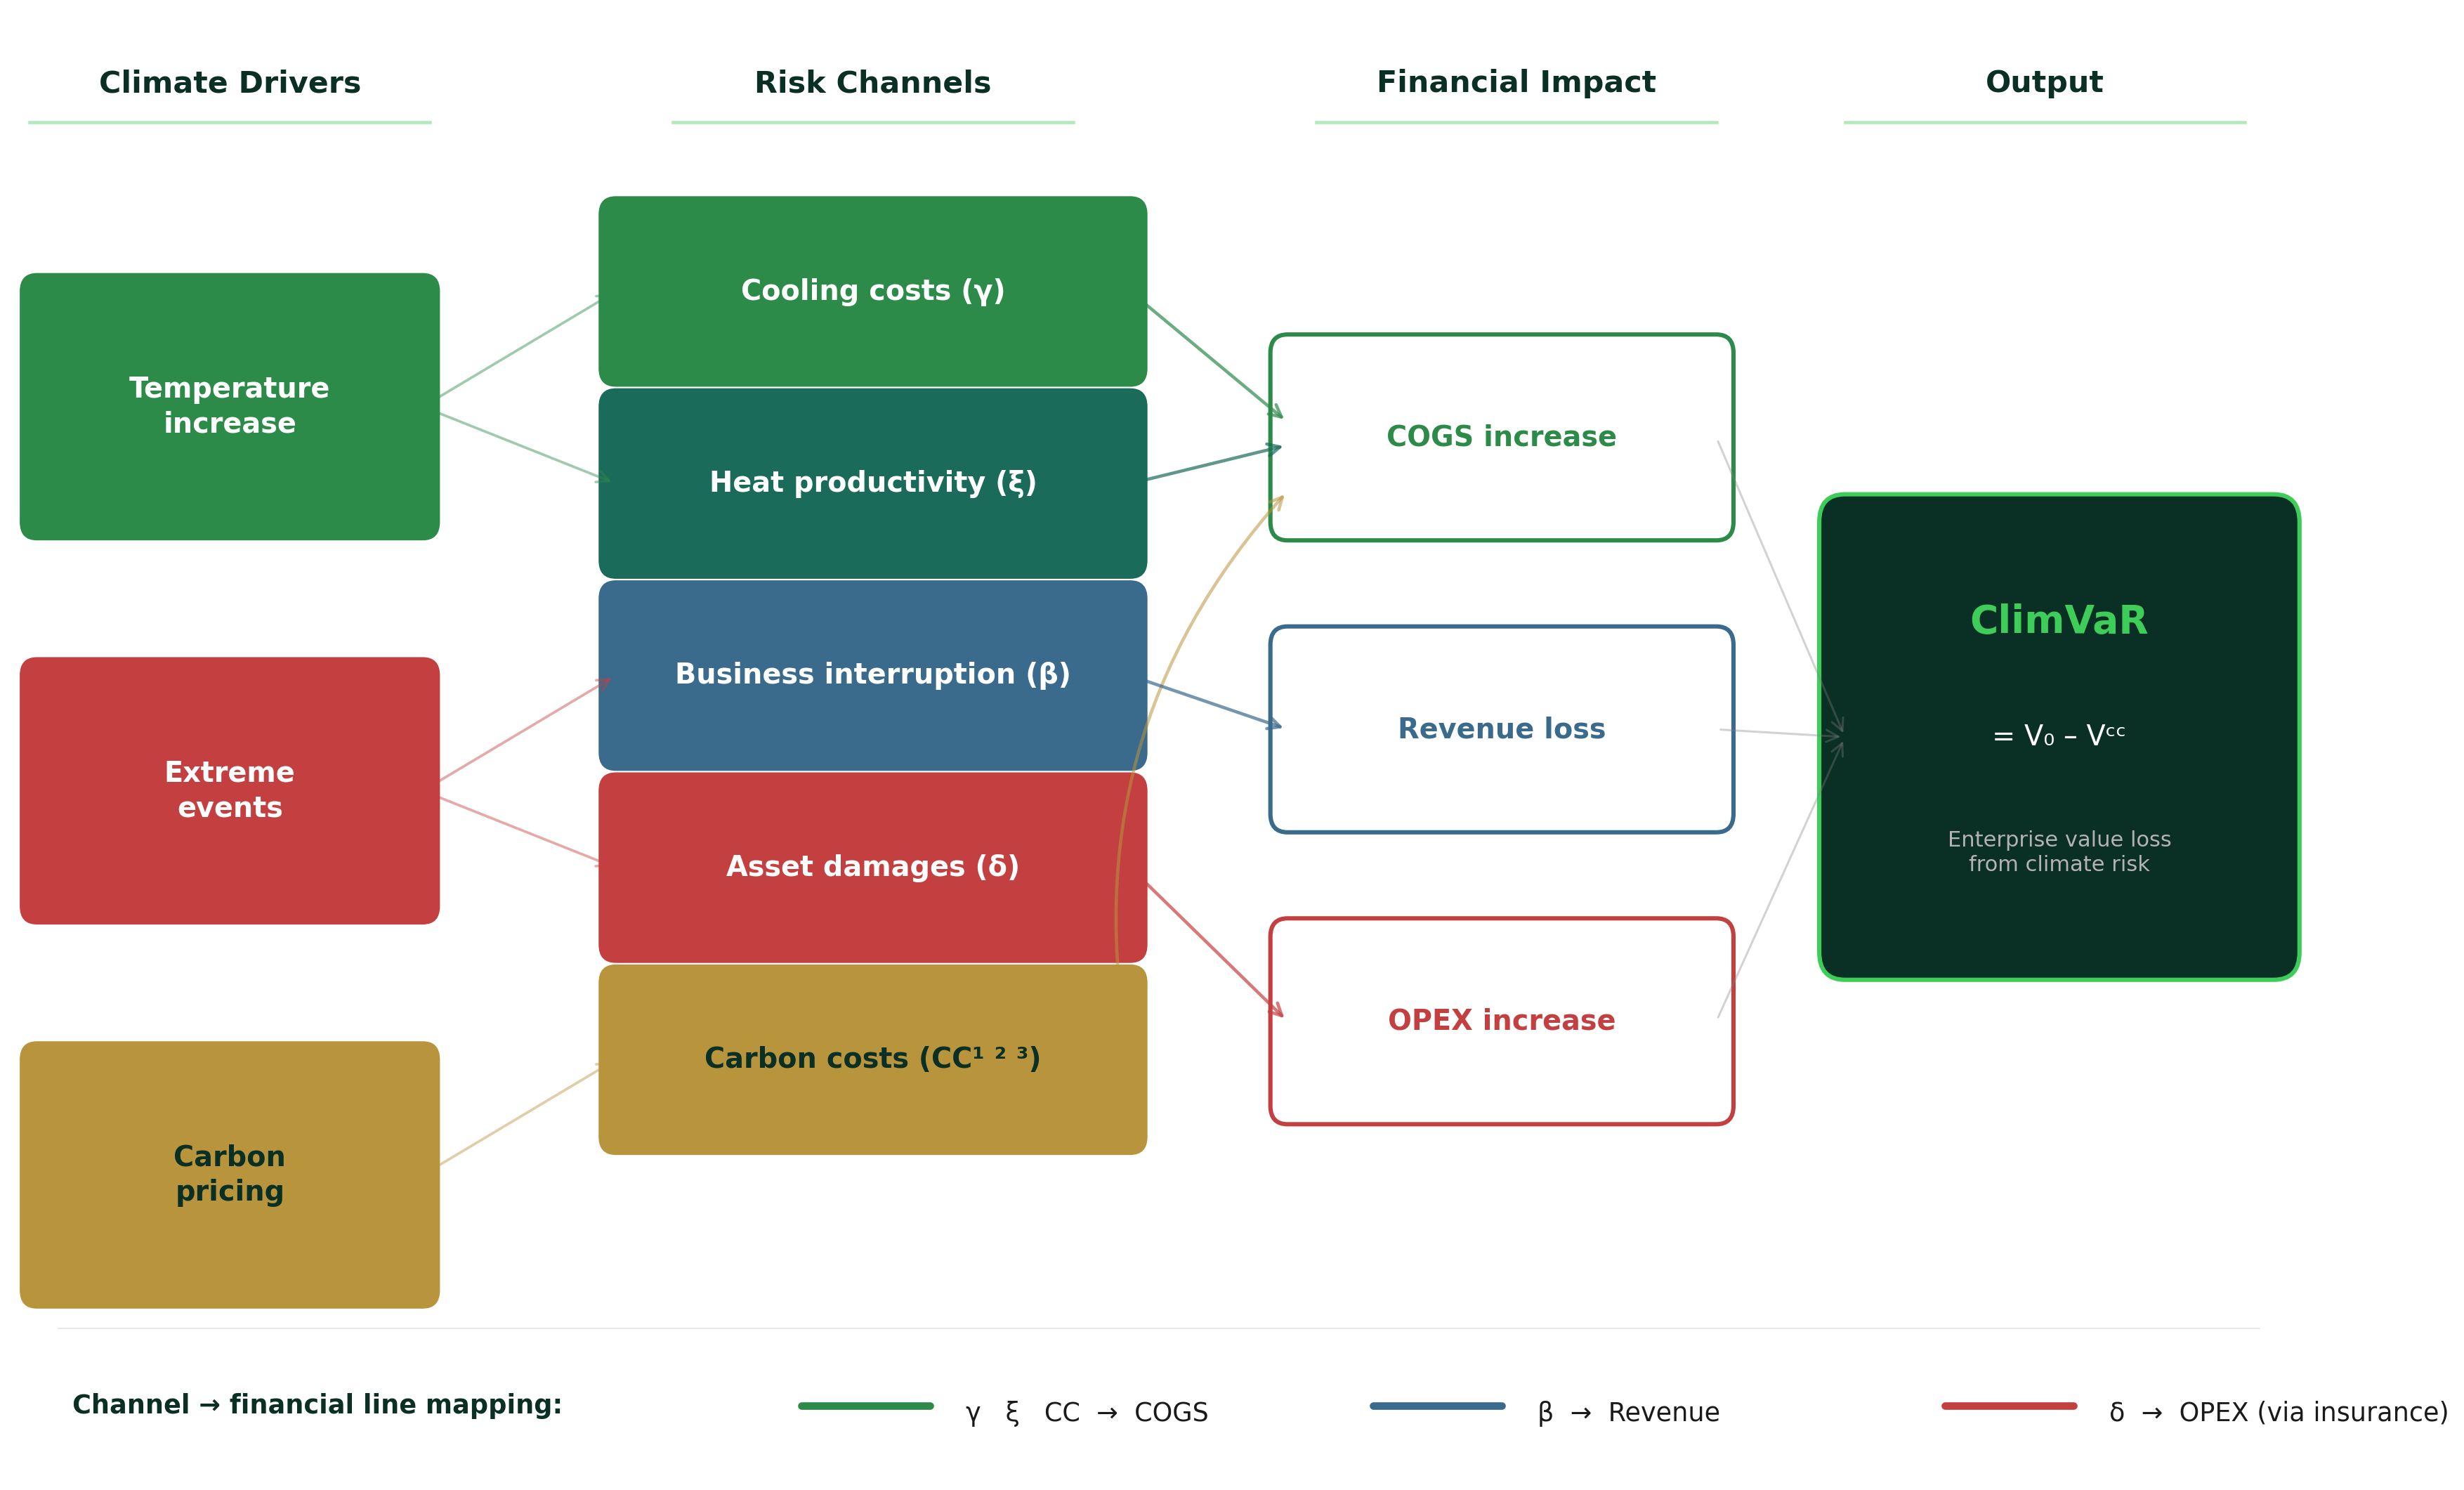
\includegraphics[width=\textwidth]{images/exhibit-framework-v2.png}
\end{center}
\exhibitsource{Adapted from Epelbaum (2025). Complete derivation in Appendix~A.}

\begin{twocolbody}

\noindent The general ClimVaR framework defines seven risk channels. Five are parameterized in this analysis. Two---customer shift ($\sigma$, capturing demand migration away from climate-exposed providers) and nature capital ($\rho$, capturing ecosystem service degradation)---remain in the mathematical architecture but are not activated due to insufficient sector-specific calibration data. Their exclusion makes the estimate conservative: both channels, if parameterized, would increase total ClimVaR. The $\rho$ channel is potentially material for facilities using evaporative cooling in water-stressed regions---a gap identified for future parameterization.

\subsubsection*{Shapley decomposition}

Business interruption aggregates exposure to multiple hazards that interact non-additively: a facility facing both drought and heat experiences correlated effects exceeding the sum of individual impacts. Simple additive decomposition produces attributions that either fail to sum to total risk or depend arbitrarily on ordering.

The Shapley value---from cooperative game theory (Nobel Prize 2012)---resolves this by averaging each hazard's marginal contribution across all possible orderings of hazard inclusion. With five hazards, exact computation requires $2^5 = 32$ coalition evaluations per facility---tractable for the full database of 8,572 sites. The decomposition satisfies four axioms simultaneously: efficiency (attributions sum to total risk), symmetry, null player (irrelevant hazards receive zero), and additivity \citep{shapley1953}. For a hazard $h$ in the set $H$ of all hazards, the Shapley value is:

\vspace{1mm}
\begin{center}
$\phi_h(v) = \displaystyle\sum_{S \subseteq H \setminus \{h\}} \frac{|S|!\,(|H|-|S|-1)!}{|H|!} \left[ v(S \cup \{h\}) - v(S) \right]$
\end{center}
\vspace{1mm}

\noindent where $v(S)$ is the business interruption cost when only hazards in coalition $S$ are active. The bracketed term is the marginal contribution of hazard $h$ given that hazards in $S$ already operate. Shapley decomposition applies \textit{within} the $\beta$ and $\delta$ channels, where hazard interactions are significant. Across channels, ClimVaR components aggregate additively through distinct cash flow lines. The formal derivation is in Appendix~A.

\subsubsection*{Supply chain propagation (Leontief)}

Facility-level analysis misses indirect exposure through upstream supply chains. A flood affecting semiconductor fabrication in Taiwan, a hurricane damaging transformer manufacturing on the Gulf Coast, or a drought constraining equipment production---all translate into business interruption for facilities thousands of kilometers distant.

Leontief input-output analysis (Nobel Prize 1973) traces this propagation using OECD\footnote{Organisation for Economic Co-operation and Development.} Multi-Regional Input-Output Tables (2023 vintage, reference year 2020) \citep{miller2009inputoutput}. The Leontief inverse captures the full cascade---not just immediate suppliers, but suppliers of suppliers. The empirical multiplier is $\times$11: for every dollar of direct business interruption, eleven dollars of supply chain value are at risk. At every facility examined, 98--99\% of business interruption risk originates upstream, not on site.

\end{twocolbody}

\begin{pullquote}
At every facility examined, 98--99\% of business interruption risk originates upstream in the supply chain, not on site. A facility's apparent geographic safety may tell little about its actual interruption exposure.
\end{pullquote}

% =====================================================================
% SECTION 2: DATABASE
% =====================================================================
\subsection*{8,572 Facilities, 120 Countries}
\greensep

\begin{twocolbody}

\noindent The core database comprises 8,572 geocoded facilities totaling 90.8~GW across 120 countries, assembled from industry databases, regulatory filings, operator disclosures, and satellite imagery validation. Each facility carries 29 documented financial parameters (revenue, asset value, cost ratios, PUE, carbon intensity, insurance). Financial calibration uses regional and tier-specific benchmarks rather than facility-specific data. Asset values range from \$5M/MW for legacy colocation in emerging markets to \$42M/MW for hyperscale AI facilities in the United States. This archetype-based approach enables full database coverage while introducing uncertainty proportional to individual facilities' divergence from their regional benchmark.

Physical risk variables are extracted from bias-corrected, statistically downscaled CMIP projections at facility-level coordinates: temperature, precipitation, wind speed, and flood depth across five hazard types (tropical wind, river flood, coastal flood, wildfire, extreme heat). The total dataset comprises approximately 50~million climate observations across two RCP pathways and the 2026--2050 horizon. Projections are sourced from multi-model ensembles; the Q25/MEAN/Q95 reporting structure in Chapter~III reflects variation from spatial heterogeneity, model sensitivity, and stochastic event occurrence.

Supply chain propagation uses the OECD Multi-Regional Input-Output Tables (2023 vintage, 75 countries $\times$ 45 sectors), with eight components extracted for the data center value chain. Carbon pricing trajectories are drawn from NGFS\footnote{Network for Greening the Financial System: a consortium of central banks and supervisors developing climate scenario frameworks.} scenarios (2023), differentiated by region and policy pathway. Grid emission factors use IEA\footnote{International Energy Agency.} country-level data (2024), with forward projections aligned to each transition scenario.

Prospective capacity represents the AI-era pipeline through 2050, modeled under three growth scenarios from \citet{paccou2024}: \textbf{Limits to Growth} (LTG, +63~GW)---where energy and resource constraints slow AI expansion; \textbf{Sustainable AI} (SAI, +121~GW)---growth within efficiency guardrails; and \textbf{Abundance Without Boundaries} (AWB, +296~GW)---compute demand scales with minimal constraint. All three are nested by construction: LTG $\subset$ SAI $\subset$ AWB. Facilities are drawn from four source pools ordered by decreasing certainty: Epoch AI GPU cluster database (62 facilities, 6.3~GW), Tier~2 announced projects (60 facilities, 6.0~GW), and two probabilistic pools allocated via regional demand models \citep{iea2025energyai, paccou2024}. Major identified projects include large-scale AI training facilities in the US South (up to 2,800~MW), next-generation GPU clusters, and sovereign AI deployments. Actual buildout will differ in timing, scale, and location; ClimVaR estimates for prospective infrastructure are indicative of the risk profile under each scenario, not point predictions.

\end{twocolbody}

\vspace{2mm}
\exhibitcaption{7a}{Facility coverage by region and AI growth scenario.}

\begin{center}
\datatablesetup
\begin{tabularx}{\textwidth}{l >{\raggedleft\arraybackslash}X >{\raggedleft\arraybackslash}X >{\raggedleft\arraybackslash}X >{\raggedleft\arraybackslash}X >{\raggedleft\arraybackslash}X >{\raggedleft\arraybackslash}X >{\raggedleft\arraybackslash}X >{\raggedleft\arraybackslash}X}
\toprule
\datatableheader
& \multicolumn{2}{c}{\thd{Installed}} & \multicolumn{2}{c}{\thd{+ Limits to Growth}} & \multicolumn{2}{c}{\thd{+ Sustainable AI}} & \multicolumn{2}{c}{\thd{+ Abundance}} \\
\rowcolor{SEGreen}
\thd{Region} & \thd{Sites} & \thd{GW} & \thd{Sites} & \thd{GW} & \thd{Sites} & \thd{GW} & \thd{Sites} & \thd{GW} \\
\midrule
United States  & 2,383 & 30.3 & 2,620 & 54.0 & 2,831 & 75.1 & 3,464 & 138.4 \\
China          & 1,284 & 25.1 & 1,395 & 36.2 & 1,522 & 48.9 & 1,902 & 86.9 \\
Europe         & 2,019 & 15.4 & 2,101 & 23.6 & 2,170 & 30.5 & 2,376 & 51.1 \\
Asia-Pacific   & 1,593 & 11.6 & 1,692 & 22.9 & 1,804 & 34.3 & 2,145 & 68.5 \\
Rest of World  & 1,293 & 8.5  & 1,379 & 17.1 & 1,440 & 23.2 & 1,624 & 41.6 \\
\midrule
\textbf{Total} & \textbf{8,572} & \textbf{90.8} & \textbf{9,187} & \textbf{153.7} & \textbf{9,767} & \textbf{212.0} & \textbf{11,511} & \textbf{386.4} \\
\bottomrule
\end{tabularx}
\datatableclear
\end{center}

\clearpage\thispagestyle{chapterstart}

\exhibitcaption{7b}{AI growth scenarios: capacity trajectories with sensitivity to system dynamics parameters.}
\begin{center}
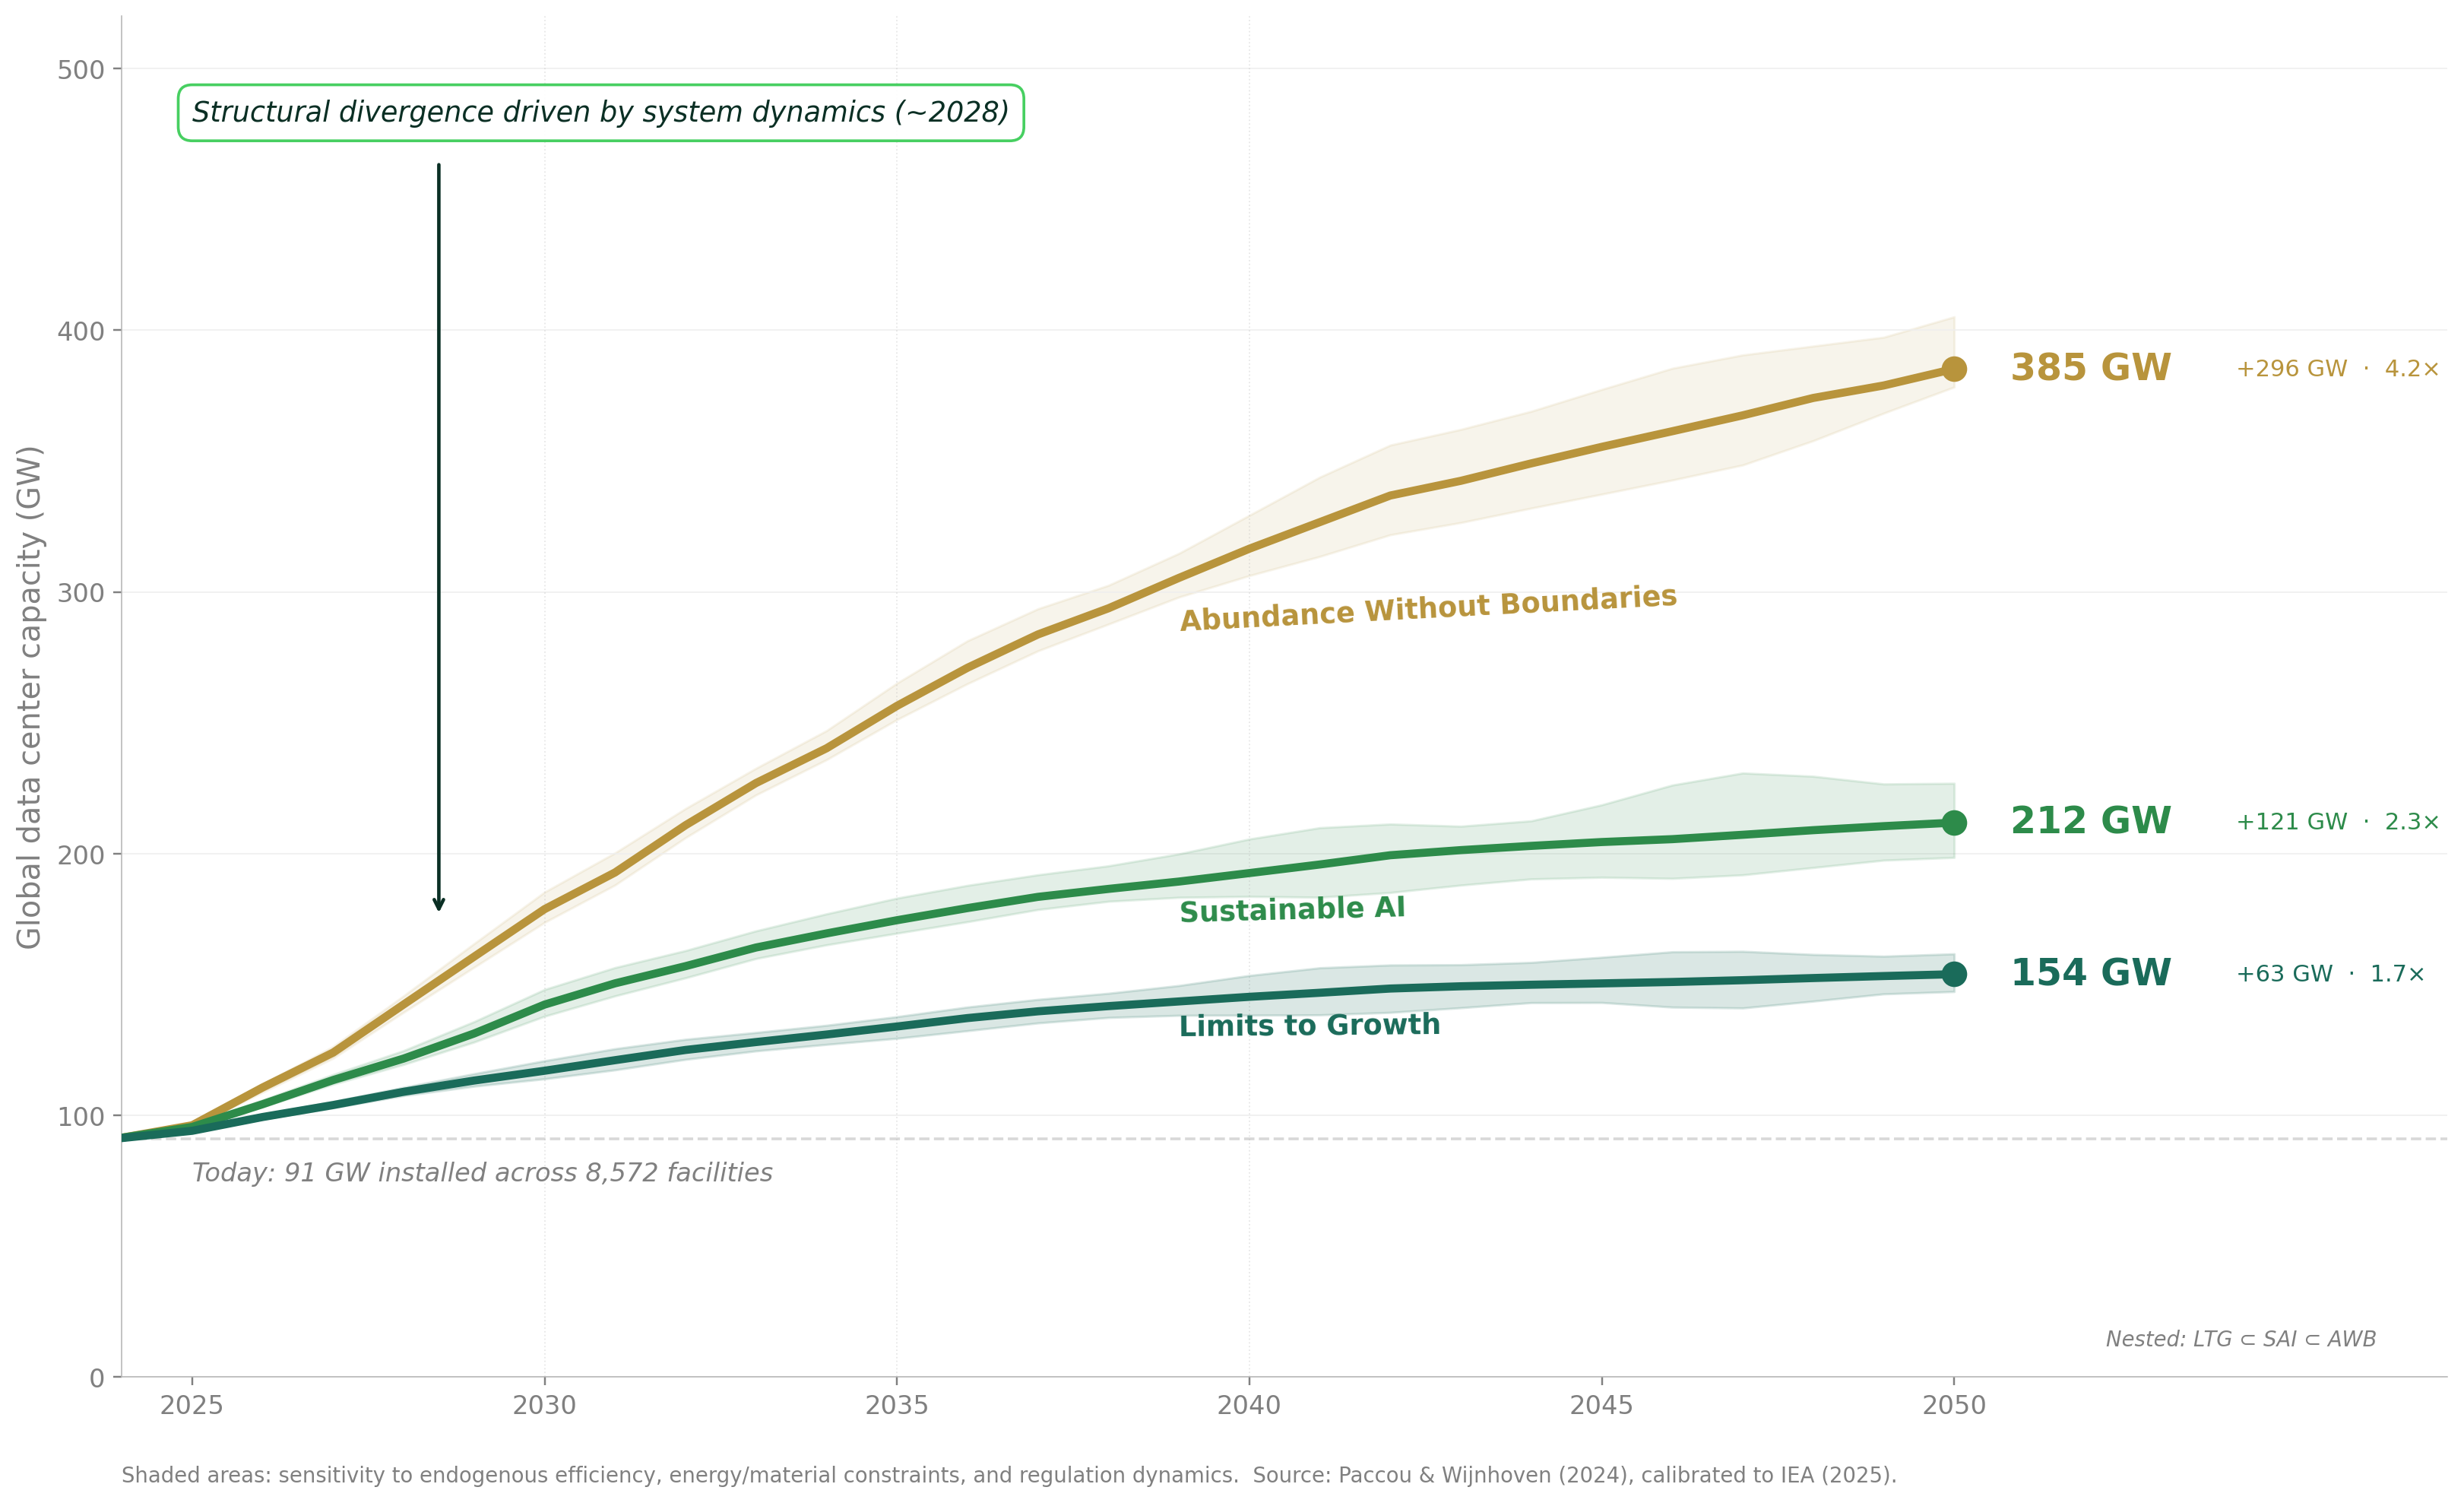
\includegraphics[width=\textwidth]{images/exhibit-scenarios-trajectories.png}
\end{center}

\begin{twocolbody}

The distinction matters for adaptation economics. Legacy facilities face locked-in exposure reducible only through costly retrofits (40--60\% of CAPEX). Prospective facilities can integrate climate resilience at the design stage---typically at 15--20\% of CAPEX. Each year without action converts a greenfield opportunity into a future retrofit cost. Of the 29 financial parameters, 48\% are calibrated from high-confidence public sources, 34\% from mixed sources, and 17\% from expert judgment. Sensitivity analysis confirms robustness to $\pm$20\% variation in expert-judgment parameters; the dominant uncertainty source is physical hazard projection, not financial calibration. The complete data architecture is documented in Appendix~B.

\end{twocolbody}

\clearpage\thispagestyle{chapterstart}

% =====================================================================
% SECTION 3: SCENARIO ARCHITECTURE
% =====================================================================

\subsection*{Four Dimensions of Uncertainty}
\greensep

\begin{twocolbody}

\noindent The analysis crosses four dimensions of uncertainty. The first two---physical pathways and transition policies---represent external uncertainty that operators cannot individually influence. The third---AI growth---determines the asset base. The fourth---adaptation---is the strategic variable.

\end{twocolbody}

\vspace{2mm}
\exhibitcaption{8}{Scenario architecture: four dimensions of uncertainty.}

\begin{center}
\datatablesetup
\begin{tabularx}{\textwidth}{>{\raggedright\arraybackslash}p{2.4cm} >{\raggedright\arraybackslash}p{2.4cm} >{\raggedright\arraybackslash}p{2.4cm} >{\raggedright\arraybackslash}X}
\toprule
\datatableheader
\thd{Dimension} & \thd{Source} & \thd{Options} & \thd{What it determines} \\
\midrule
Physical pathway & IPCC (RCP) & 2.6 / 8.5 & Temperature trajectories, extreme event frequency, flood probabilities \\
Transition policy & NGFS & BAU / Net Zero & Carbon price trajectories, grid decarbonization pace \\
AI growth & Paccou \& Wijnhoven (2024) & LTG / SAI / AWB & Scale and geography of infrastructure deployment \\
Adaptation strategy & Operator choice & Baseline / Selective / Proactive & Technology, siting, and retrofit decisions \\
\bottomrule
\end{tabularx}
\datatableclear
\end{center}

\begin{twocolbody}

\subsubsection*{Physical pathways}

Representative Concentration Pathways (RCPs)\footnote{RCPs are greenhouse gas concentration trajectories adopted by the IPCC for climate modelling. RCP~2.6 is consistent with the Paris Agreement; RCP~8.5 represents unabated emissions.} determine the physical hazard environment---temperature trajectories, extreme event frequencies, flood and storm probabilities---which operators cannot influence individually. Two endpoints bracket the range from Paris-aligned mitigation to unabated emissions.

\end{twocolbody}

\vspace{2mm}
\exhibitcaption{9}{Physical climate scenarios and data center implications.}

\begin{center}
\datatablesetup
\begin{tabularx}{\textwidth}{>{\raggedright\arraybackslash}p{2.8cm} >{\raggedright\arraybackslash}p{2.5cm} >{\raggedright\arraybackslash}p{3cm} >{\raggedright\arraybackslash}X}
\toprule
\datatableheader
\thd{Scenario} & \thd{Warming by 2100} & \thd{Implied policy} & \thd{DC-relevant implications} \\
\midrule
RCP 2.6 / SSP1-2.6 & +1.5--2.0$^\circ$C & Paris Agreement met & Cooling costs +15--25\%; extreme events +20--40\% \\
RCP 8.5 / SSP5-8.5 & +4.0--5.0$^\circ$C & No mitigation & Cooling costs +35--50\%; extreme events +100--200\% \\
\bottomrule
\end{tabularx}
\datatableclear
\end{center}
\exhibitsource{RCPs drive physical risk channels: $\gamma$ (cooling), $\beta$ (extreme events), $\delta$ (damage), and $\xi$ (heat exposure). Downscaled from CMIP ensemble \citep{eyring2016}.}

\begin{twocolbody}

\subsubsection*{Transition policies and adaptation}

Transition policies cross physical pathways with carbon pricing trajectories. Under BAU, carbon prices follow current legislated trajectories. Under Net Zero Transition (NZT), prices rise to levels consistent with NGFS net-zero-by-2050 scenarios \citep{ngfs2023}. NZT \textit{increases} installed base ClimVaR (from 38\% to 83\%) because higher carbon prices amplify the CC channel---a counter-intuitive result with direct implications for operators whose sustainability strategy relies on transition risk declining over time.

Three adaptation strategies are modeled. \textbf{Baseline}: current practice, no additional climate investment. \textbf{Selective}: targeted intervention on the highest-Shapley-value channel per facility---the ``one champion action'' approach. \textbf{Proactive}: comprehensive investment across all five channels. Risk reductions across channels are multiplicative, not additive, because the channels interact through the Shapley structure.

Three AI growth scenarios bracket deployment uncertainty \citep{paccou2024}. \textbf{Limits to Growth (LTG)}: energy and resource constraints slow AI expansion (+63~GW). \textbf{Sustainable AI (SAI)}: growth within efficiency guardrails (+121~GW). \textbf{Abundance Without Boundaries (AWB)}: compute demand scales with minimal constraint (+296~GW). All three are nested by construction: LTG $\subset$ SAI $\subset$ AWB.

\subsubsection*{Intra-scenario uncertainty}

Within each scenario combination, results are reported at three statistical levels to characterize the distribution of outcomes: \textbf{Q25} (25th percentile---optimistic estimate), \textbf{MEAN} (expected value across the facility distribution---the central estimate used for most results), and \textbf{Q95} (95th percentile---tail risk estimate). This allows distinguishing between expected outcomes and tail risks that drive insurance pricing and capital allocation decisions. The Q25--Q95 range reflects variation from spatial heterogeneity, firm-level differences in carbon intensity, and stochastic event occurrence. Unless noted otherwise, all results in Chapter~III use the BAU/MEAN pathway.

\end{twocolbody}